\section{Objektorientierte Analyse}\label{analyse}
Im Zuge des Kapitels Analyse wird der Prototyp und das verwendete SAP UI5 Framework analysiert und die Ergebnisse in Form von Diagrammen gezeigt und beschrieben. Beginnend werden die Kombinationsmöglichkeiten zwischen den einzelnen Bibliotheken des SAP UI5 Frameworks aufgezeigt. Im Anschluss kommt eine Verdeutlichung eines Nachrichtenflusses innerhalb der SAP UI5 Applikation.

\subsection{Bibliotheken Beziehungen}
// Lib Diagramm beschreiben

\vspace{1em}
\begin{figure}[htb]
  \centering
  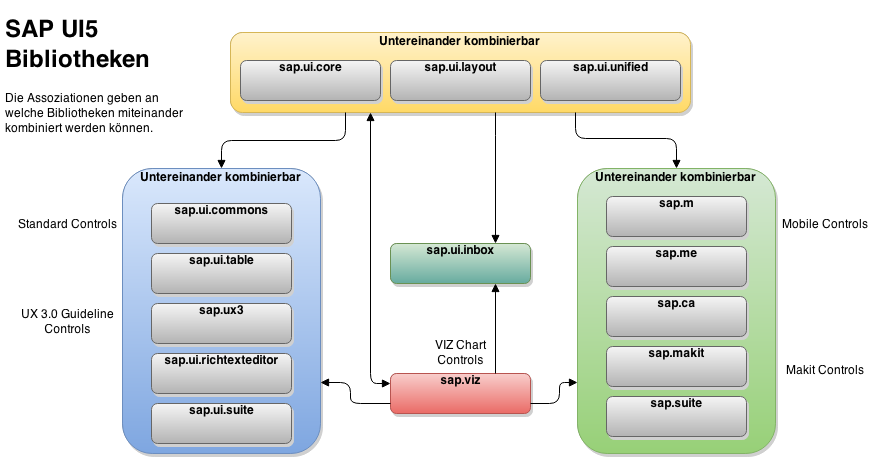
\includegraphics[width=1\linewidth]{abb/sapui5libconnections}
  \caption[SAP UI5 Bibliotheken Kombinationen]{SAP UI5 Bibliotheken Kombinationen}
  \label{fig:sapui5libconnections}
\end{figure}

// Komponentendiagramm erstellen und beschreiben

\subsection{Nachrichtenfluss}
// Sequenzdiagramm erstellen und beschreiben

\subsection{PLATZHALTER}
// Datenflussdiagramm erstellen und beschreiben
// oder anderes gutes Diagramm